\documentclass{article}
\usepackage{amsmath}
\usepackage{amssymb}
\usepackage{graphicx}
\usepackage{hyperref}
\usepackage[version=4]{mhchem}

\title{Problem 11}
\date{}

\begin{document}
\maketitle

\section*{Problem}
Two parallel chords on the same side of the center of a circle are 12 inches and 20 inches long and 2 inches apart. Find the radius of the circle. Express your answer in simplest radical form.

\section*{Solution}
\(5 \sqrt{13\).}
Let \(r\) be the radius of the circle. \(A \mathrm{~B}=10 . A D=6 . C F=20\). \(C E=10 . D E=2 . O E=x\).\\
\centering
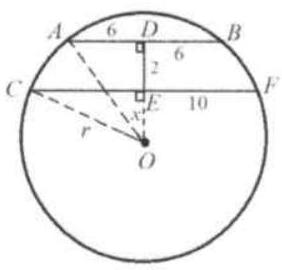
\includegraphics[width=\textwidth]{images/160(3).jpg}

Applying Pythagorean Theorem to right triangles \(A D O\) and\\
CEO: \(A D^{2}+D O^{2}=C E^{2}+O E^{2} \quad \Rightarrow\)\\
\(6^{2}+(2+x)^{2}=10^{2}+x^{2} \quad \Rightarrow x=15\).\\
\(r=\sqrt{C E^{2}+O E^{2}}=\sqrt{10^{2}+15^{2}}=5 \sqrt{13}\).

\end{document}
